\documentclass[tikz, border=8pt]{standalone}
\usepackage[T1]{fontenc}
\usepackage{tgpagella}
\usepackage{mathpazo}
\usepackage{tikz}
\usepackage{amsmath}
\usepackage{amssymb}
\usepackage{xcolor}
\usepackage{fontawesome5}
\usetikzlibrary{positioning, arrows.meta, shapes.geometric, fit, backgrounds, calc}

% ----------------------------------------------------------------
% Inline palette -- mirrors figures/_palette.tex (AGENTS.md rule 1).
% ----------------------------------------------------------------
\definecolor{cAudio}{HTML}{F5EFE3}
\definecolor{cEnc}{HTML}{DDE9EC}
\definecolor{cEncB}{HTML}{2D8294}
\definecolor{cAdp}{HTML}{F0DFC9}
\definecolor{cAdpB}{HTML}{B07849}
\definecolor{cLLM}{HTML}{F4E6D5}
\definecolor{cLLMB}{HTML}{A0763C}
\definecolor{cPrompt}{HTML}{F1ECE3}
\definecolor{cPromptB}{HTML}{8E7A55}
\definecolor{cTok}{HTML}{E5EEF0}
\definecolor{cTokB}{HTML}{5E8090}
\definecolor{cBound}{HTML}{ECDFD3}
\definecolor{cBoundB}{HTML}{9C7558}

\tikzset{
  pstep/.style     ={draw, rounded corners=3pt, align=center,
                     line width=0.75pt, fill=cEnc, draw=cEncB,
                     minimum width=9.0cm, minimum height=1.1cm,
                     font=\small, inner sep=4pt},
  outbox/.style    ={draw, rounded corners=3pt, align=center,
                     line width=0.85pt, fill=cAdp, draw=cAdpB,
                     minimum width=9.0cm, minimum height=1.0cm,
                     font=\small, inner sep=4pt},
  callout/.style   ={draw, rounded corners=2.5pt, align=center,
                     line width=0.55pt, fill=cAudio, draw=black!40,
                     minimum width=4.7cm, minimum height=1.1cm,
                     font=\scriptsize, inner sep=3.5pt},
  negbox/.style    ={draw, dashed, rounded corners=3pt, align=center,
                     line width=0.7pt, fill=cTok!28, draw=cTokB,
                     minimum width=14.6cm, minimum height=1.3cm,
                     font=\small, inner sep=4pt},
  flow/.style      ={-Stealth, line width=0.8pt, draw=black!72},
  uses/.style      ={densely dotted, line width=0.7pt, draw=black!45},
}

% --- step body: bold title + scriptsize detail row, in a minipage ---
\newcommand{\stepbody}[2]{%
  \begin{minipage}[c]{8.4cm}\centering%
    \textbf{#1}\\[1.5pt]%
    {\scriptsize\color{black!70}#2}%
  \end{minipage}%
}
\newcommand{\calloutbody}[2]{%
  \begin{minipage}[c]{4.3cm}\centering%
    \textbf{\scriptsize #1}\\[1pt]%
    {\scriptsize\color{black!72}#2}%
  \end{minipage}%
}

\begin{document}
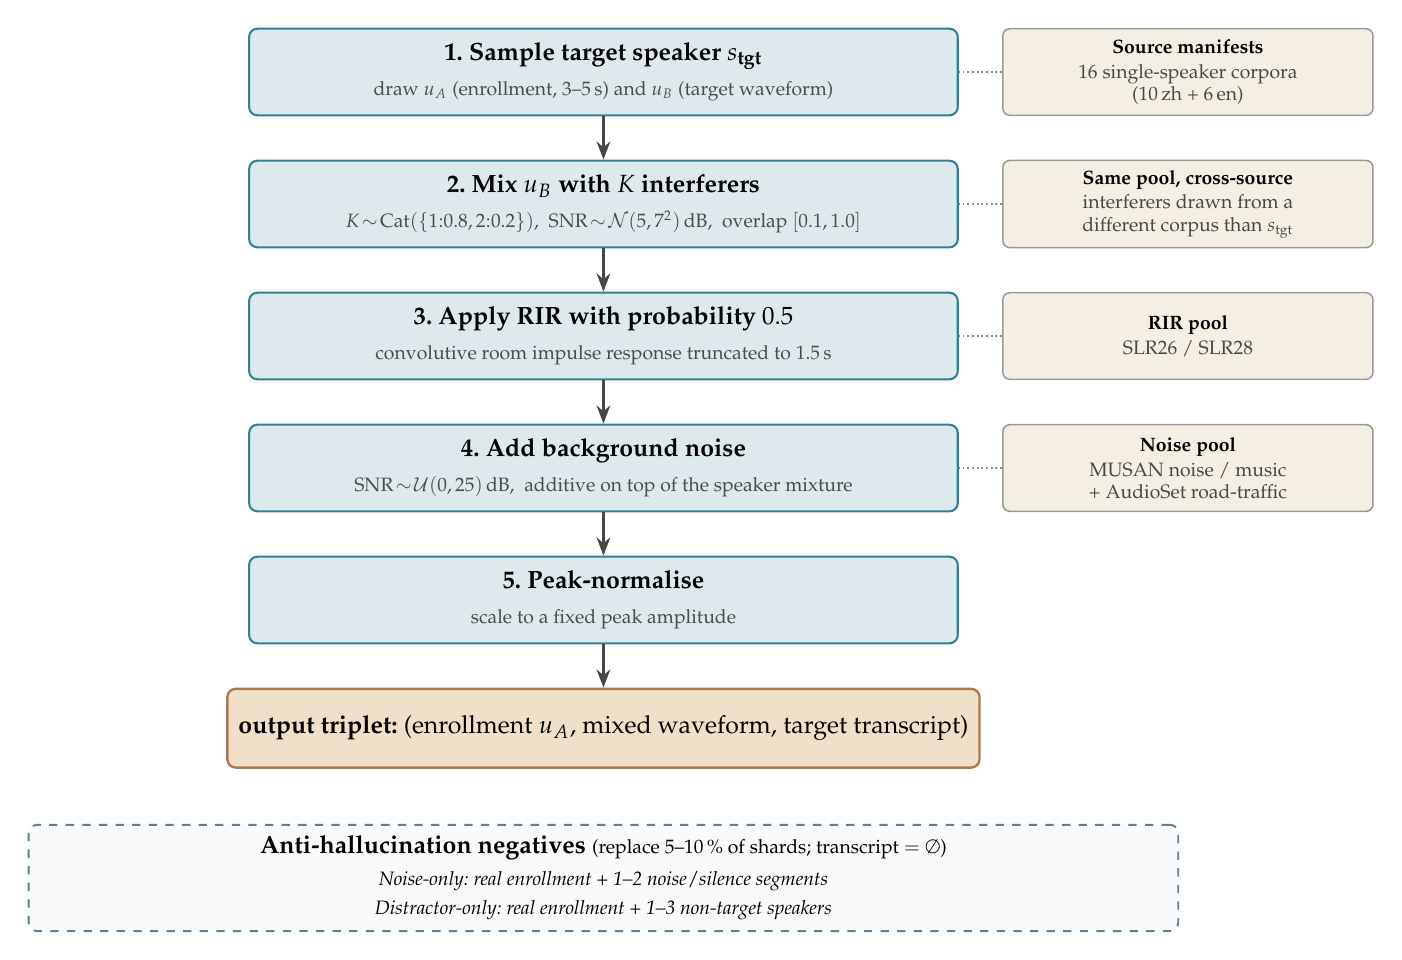
\begin{tikzpicture}[node distance=0.55cm and 0.55cm]

  % ============================================================
  % MAIN PIPELINE (left column, vertical 5 steps + output)
  % ============================================================
  \node[pstep] (step1)
    {\stepbody{1.~Sample target speaker $s_\text{tgt}$}
              {draw $u_A$ (enrollment, 3--5\,s) and $u_B$ (target waveform)}};
  \node[pstep, below=of step1] (step2)
    {\stepbody{2.~Mix $u_B$ with $K$ interferers}
              {$K\!\sim\!\mathrm{Cat}(\{1{:}0.8,2{:}0.2\})$,~
               $\mathrm{SNR}\!\sim\!\mathcal{N}(5,7^2)\,$dB,~
               overlap $[0.1, 1.0]$}};
  \node[pstep, below=of step2] (step3)
    {\stepbody{3.~Apply RIR with probability $0.5$}
              {convolutive room impulse response truncated to $1.5\,$s}};
  \node[pstep, below=of step3] (step4)
    {\stepbody{4.~Add background noise}
              {$\mathrm{SNR}\!\sim\!\mathcal{U}(0,25)\,$dB,~
               additive on top of the speaker mixture}};
  \node[pstep, below=of step4] (step5)
    {\stepbody{5.~Peak-normalise}
              {scale to a fixed peak amplitude}};

  \node[outbox, below=0.55cm of step5] (output)
    {\textbf{output triplet:}~(enrollment $u_A$,~mixed waveform,~target transcript)};

  % --- Main-flow vertical arrows ---
  \draw[flow] (step1) -- (step2);
  \draw[flow] (step2) -- (step3);
  \draw[flow] (step3) -- (step4);
  \draw[flow] (step4) -- (step5);
  \draw[flow] (step5) -- (output);

  % ============================================================
  % RESOURCE CALLOUTS (right column, one per consuming step)
  % Short dotted attachments only -- no top-row swim lane.
  % ============================================================
  \node[callout, right=of step1] (r1)
    {\calloutbody{Source manifests}
                 {16 single-speaker corpora\\(10\,zh + 6\,en)}};
  \node[callout, right=of step2] (r2)
    {\calloutbody{Same pool, cross-source}
                 {interferers drawn from a\\different corpus than $s_\text{tgt}$}};
  \node[callout, right=of step3] (r3)
    {\calloutbody{RIR pool}
                 {SLR26 / SLR28}};
  \node[callout, right=of step4] (r4)
    {\calloutbody{Noise pool}
                 {MUSAN noise / music\\+ AudioSet road-traffic}};

  \draw[uses] (r1.west) -- (step1.east);
  \draw[uses] (r2.west) -- (step2.east);
  \draw[uses] (r3.west) -- (step3.east);
  \draw[uses] (r4.west) -- (step4.east);

  % ============================================================
  % ANTI-HALLUCINATION BRANCH (bottom, independent block)
  % No flow arrow into / out of it -- caption explains the
  % 5--10\,\% shard-replacement semantics.
  % ============================================================
  \node[negbox, below=0.7cm of output] (neg) {%
    \textbf{Anti-hallucination negatives}~%
    {\scriptsize (replace 5--10\,\% of shards;~transcript $=\emptyset$)}\\[0.5pt]
    {\scriptsize\itshape Noise-only:~real enrollment + 1--2 noise\,/\,silence segments}\\[-0.5pt]
    {\scriptsize\itshape Distractor-only:~real enrollment + 1--3 non-target speakers}};

\end{tikzpicture}
\end{document}
